\documentclass[12pt,letterpaper,titlepage]{article}

\usepackage{fontspec}
\defaultfontfeatures{Mapping=tex-text}
\usepackage{xunicode}
\usepackage{xltxtra}
\usepackage{amsmath}
\usepackage{pdfpages}
\usepackage{mathtools}
\usepackage{amsfonts}
\usepackage{amssymb}
\setcounter{secnumdepth}{0}
\usepackage{nameref}
\usepackage{enumitem}
\usepackage{environ}

\showboxdepth=\maxdimen
\showboxbreadth=\maxdimen

\usepackage[tocflat]{tocstyle}
\usetocstyle{allwithdot}
\usepackage[bottom]{footmisc}

\usepackage{paracol}
\usepackage{wrapfig}
\globalcounter{table}
\globalcounter{figure}
\usepackage{graphicx}
\usepackage[left=1in,right=1in,top=1in,bottom=1in]{geometry}
\graphicspath{{img/}}

\author{Jacob Abel}
\title{	Homework 3
	\\\large MATH2534 CRN:15708
}

\setlength{\parskip}{0.5em}

\begin{document}
\maketitle
\begin{raggedright}

\begin{enumerate}
\item Consider $D = \mathbb{Q}$ as the domain of the predicate variables $x$ and $y$. Discern which of the following statements are true and which are false. Give counterexamples for the statements which are false.

  \begin{enumerate}[label=(\alph*)]
    \item $x > 0$ and $y < 0 \implies x − y^2 > 0$

	  False in the case of $|x| >= |y|$    
    
    \item $xy = 0 \iff x = 0$

	  True    
    
    \item $\forall x$, $y \geq 2$, $2xy > x + y$
    
	  False in the case of $x \leq 0$
    
  \end{enumerate}
  
%=================================================================================================%

\item Put the following statements into symbolic logic using multiple quantifiers. Negate each statement.

  \begin{enumerate}[label=(\alph*)]
    \item Some colors are loved by everyone.

	  $\exists x \in$ Colours, $\forall y \in$ People $| x$ is loved by $y$
	  
	  Negate: $\forall x \in $Colours, $\exists y \in$ People $| x$ is not loved by $y$

    \item There are some students who get an A on all classes.

	  $\exists x \in$ Students, $\forall y \in$ Classes $| x$ get an A in $y$

	  Negate: $\forall x \in$ Students, $\exists y \in$ Classes $| x$ does not get an A in $y$

    \item Everyone is loved by someone.

	  $\forall x \in$ People, $\exists y \in$ People $| x$ is loved by $y$
	  
	  Negate: $\exists x \in$ People, $\forall y \in$ People $| x$ is not loved by $y$

    \item No movie will please everyone.

	  $\exists x \in$ Movies, $\forall y \in$ People $| x$ will not please $y$
	  
	  Negate: $\forall x \in$ Movies, $\exists y \in$ People $| x$ will please $y$

  \end{enumerate}
  
%=================================================================================================%

\item Write the negation, contrapositive, converse and inverse of the following statements.

  \begin{enumerate}[label=(\alph*)]
    \item For all sport cars $x$, $x$ is expensive.

	  Negation: There exists a sports car $x$, $x$ is not expensive.
	  
	  Contrapositive: For all non-expensive cars $x$, $x$ is not a sports car. 
	  
	  Converse: For all expensive cars $x$, $x$ is a sports car.
	  
	  Inverse: For all non-sport cars $x$, $x$ is not expensive.
    
    \item $\forall x \in R^+$, if $x^2 < 1$, then $x < 1$.
    
   	  Negation: $\exists x \in R^+$, $x^2 < 1 \land x \geq 1$.
	  
	  Contrapositive: $\forall x \in R^+$, if $x \geq 1$, then $x^2 \geq 1$
	  
	  Converse: $\forall x \in R^+$, if $x < 1$, then $x^2 < 1$
	  
	  Inverse: $\forall x \in R^+$, if $x^2 \geq 1$, then $x \geq 1$

  \end{enumerate}
  
%=================================================================================================%
\pagebreak

\item Write the following statements as quantified conditional statements; if-then form.

  \begin{enumerate}[label=(\alph*)]
    \item Driving over 70 miles per hour is a sufficient condition for getting a ticket.
    
	  $\forall x \in$ Vehicles $|$ if $x$ is moving faster than 70 mph, then $x$ receives a ticket.
    
    \item Being responsible is a necessary condition for being a president for the club.

	  $\forall x \in $People $|$ if $x$ is not responsible, then $x$ cannot be president for the club.

  \end{enumerate}

%=================================================================================================%

\item Let $A = B = \{−5, −2, 2, 4, 6, 8, 12, 15\}$. Determine whether the given statement is true and write a negation for each statement.

  \begin{enumerate}[label=(\alph*)]
    \item $\forall x \in A$, $\exists y \in B$ such that $x + y = 10$.

	  True
	  
	  Negation: $\exists x \in A$, $\forall y \in B$ such that $x + y \neq 10$.
    
    \item $\exists x \in A$ such that $\forall y \in B, x \geq y^2$.
    
	  False

	  Negation: $\forall x \in A$ such that $\exists y \in B, x < y^2$.
    
  \end{enumerate}

%=================================================================================================%

\item
Domain D: VT students 

Domain E: VT football games 

Predicate: $P(x, y) = x$ watches $y$. 

Write the following symbolic statements and negations in conventional English:

  \begin{enumerate}[label=(\alph*)]
    \item $\forall y \in E$, $\exists x \in D$ such that $P(x, y)$.
    
	  All VT football games have VT students watching them.    

    \item $\exists x \in D$ such that $\forall y \in E$, $P(x, y)$.

	  There are VT students that watch all VT football games.

    \item $\exists y \in E$ such that $\forall x \in D$, $P(x, y)$.

	  There are VT football games that all VT students watch.

    \item $\forall x \in D$, $\exists y \in E$ such that $P(x, y)$.

	  All VT students watch some VT football game.

  \end{enumerate}

%=================================================================================================%
\pagebreak

\item This problem refers to Example 3.3.3 in the textbook or Example 2, 3.3 in lecture notes.

\begin{center}
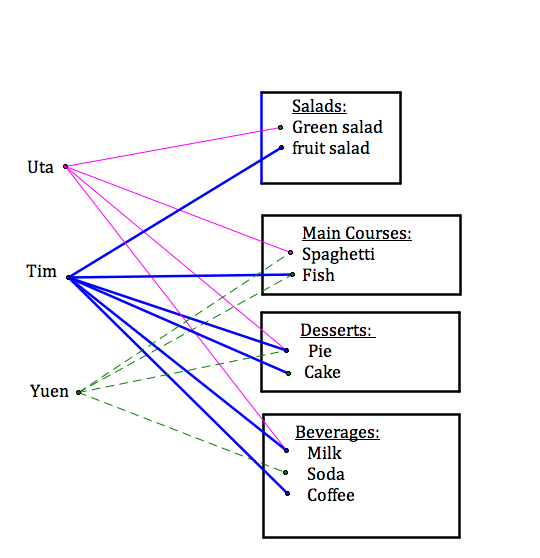
\includegraphics[width=.5\textwidth, height=\textheight, keepaspectratio=true]{hw3q7}
\end{center}

Write each of following statements informally and find its truth value.

  \begin{enumerate}[label=(\alph*)]
    \item $\forall$ students $S$, $\exists$ a salad $I$ such that $S$ chose $I$.
    
	  All students chose a salad.   
    
    \item $\forall$ items $I$, $exists$ a student $S$ such that $S$ did not choose $I$.

	  All items were not chosen by some student.

	  False

    \item $\exists$ a student $S$ such that $\exists$ a station $Z$ such that $S$ chose $∀$ items $I$ in $Z$.

	  There is a student that chose all items at a station.
	  
	  True

    \item $\exists$ a station $Z$ such that $\forall$ students $S$, $∃$ an item $I$ such that $S$ chose $I$ in $Z$.

	  There is a station that all students chose an item from.
	  
	  True

  \end{enumerate}

%=================================================================================================%
\pagebreak

\item Use a diagram and argument forms from class, to discern whether or not the following argument is valid.

  \begin{enumerate}[label=(\alph*)]
    \item All children play a video game. 
    
    	  Paul is not a child. 
    
          $\therefore$ Paul does not play a video game.
           
      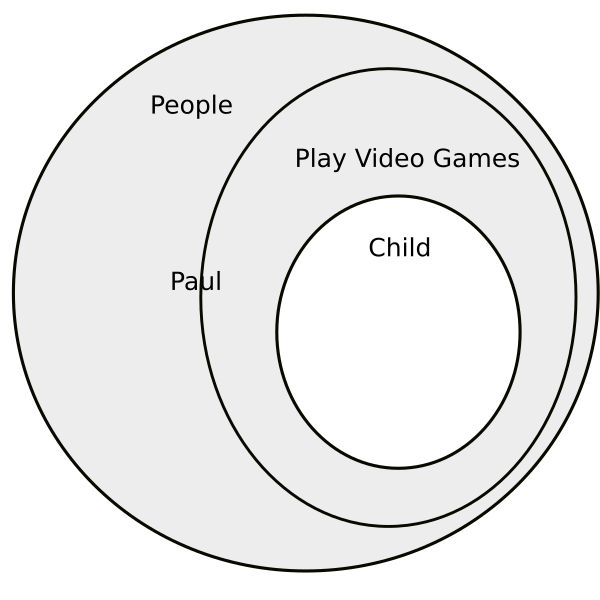
\includegraphics[width=.375\textwidth, height=\textheight, keepaspectratio=true]{hw3q8a}

	  Child $\implies$ plays a video game.
	  
	  $\neg$ Child
	  
	  $\therefore\;\neg$Plays Video Games

	  False by Inverse Error
                    
    \item No healthy food tastes good. 

    	  Candies taste good. 
    	  
    	  $\therefore$ Candies are not healthy food.
    	  
          
\includegraphics[width=.375\textwidth, height=\textheight, keepaspectratio=true]{hw3q8b}

		  Healthy $\implies\;\neg$ Tastes good

		  Taste Good
		  
		  $\therefore$ Not healthy
		  
		  True by Modus Tollens

  \end{enumerate}

\end{enumerate}
\end{raggedright}
\end{document}
